\documentclass[runningheads]{llncs}

\usepackage{amsmath}
\usepackage{url}
\usepackage{graphicx}
\usepackage{salgorithm}

\newcommand{\newword}[1]{{\bf #1}}
\newcommand{\NP}{\ensuremath{\mathcal{NP}}}
\newcommand{\Instance}{{\sc Instance~}}
\newcommand{\Question}{~\\
{\sc Question~}}
\spnewtheorem{prob}[theorem]{Problem}{\bfseries}{\itshape}

\title{Using Cell Phone Keyboards is (\NP) Hard}
\author{Peter Boothe}
\institute{Manhattan College\\
\email{peter.boothe@manhattan.edu}
}

\begin{document}
\maketitle

\begin{abstract}
Sending text messages on cell phones which only contain the keys 0-9 and \# and
* can be a painful experience.  We consider the problem of designing an optimal
mapping of numbers to sets of letters to act as an alternative to the standard
$\{2\to\{abc\}, 3\to\{def\}\ldots\}$.  Our overall goal is to minimize the
number of buttons that must be pressed to enter an aferage message in English.
We prove that the problem in almost all of its variations is \NP\ hard, but
describe several mappings which improve the standard one.  With luck, one of
these new mappings will achieve success similar to that of the Dvorak layout
for computer keyboards.
\end{abstract}

Typing on a keyboard which has fewer keys than there are letters in the
alphabet can be a painful task.  There are a plethora of input schemes which
attempt to make this task easier, but the one thing they all have in common is
that all of these input methods use the standard mapping of numeric keys to
alphabetic numbers of 
$\{2\to\{abc\},
         3\to\{def\}, 4\to\{ghi\}, 5\to\{jkl\}, 6\to\{mno\}, 7\to\{pqrs\},
         8\to\{tuv\}, 9\to\{wxyz\}\}$.
In this paper, we consider schemes of rearranging the numbers on the keys to
make messages easier to type.  Most variants of this problem turn out to be
NP-hard, unfortunately.

Before we get any farther, let us sketch the basic problem that we will keep
revising and revisiting throughout this paper.
\begin{prob}[{\sc MinimumKeystrokes}]~\\
\Instance\ A set of letters corresponding to an alphabet $A$ $(|A| =
n)$, a number of keys $k$, an input method $\mathrm{IN}$, and a set of
tuples of words and frequencies $W$.  The frequencies in $W$ are integers,
and the words are made up of solely of elements of $A$.  We will
treat $IN$ as a function which, given a partition of $A$ and a word
$w$, returns how many keystrokes are required to type $w$.

\Question\ What is the best partition of $A$ into $k$ sets, such that the
total number of keystrokes to type every word in $W$ its associated frequency
times is minimized?  Equivalently, what is the partition of $P$ of $A$ ($|P| = k$) that
will minimize
$$\sum_{(w,f)\in W} f*\mathrm{IN}(w,P)$$
\label{probtemplate}
\end{prob}


Over the course of this paper we consider three different real-world
schemes for $\mathrm{IN}$ (basic typing, T9, and predictive T9), and for each
variant that is proven \NP-hard, we consider the restriction on $P$ that
requires that we keep the alphabet in alphabetical order.  In all cases
where it is computationally feasible we provide results for the case of
the English language, on 8-key keyboards, using the British National
Corpus\cite{bnc} (BNC).  One feature of note is that no matter what scheme we
use, the problem is trivial if the number of keys is not smaller than the
number of letters in the alphabet ($k \ge |A|$).  Using tiny keyboards is only
(computationally) difficult when the keyboards don't have enough keys.

\section{Setting a Baseline with the Easiest Problem}

The baseline we compare against is the most painful method of text entry.  I
imagine that no ``digital native'' actually uses this input method, and that it
is available on all phones solely that their parents might use it.  In this
method, to type an `a', the user of the cellphone types the `2' key; to type a
`b' they type `22', to type `c' they type `222', to type a `d' they type `3',
to type an `e' they type `33', and so on.  To type a word with multiple
letters that use the same key, such as `accept', the user must pause
between keystrokes.  Thus, the full key entry sequence for `accept', using
`.' to indicate a pause, is `2.22.223378'.

\begin{figure}[t]
\begin{center}
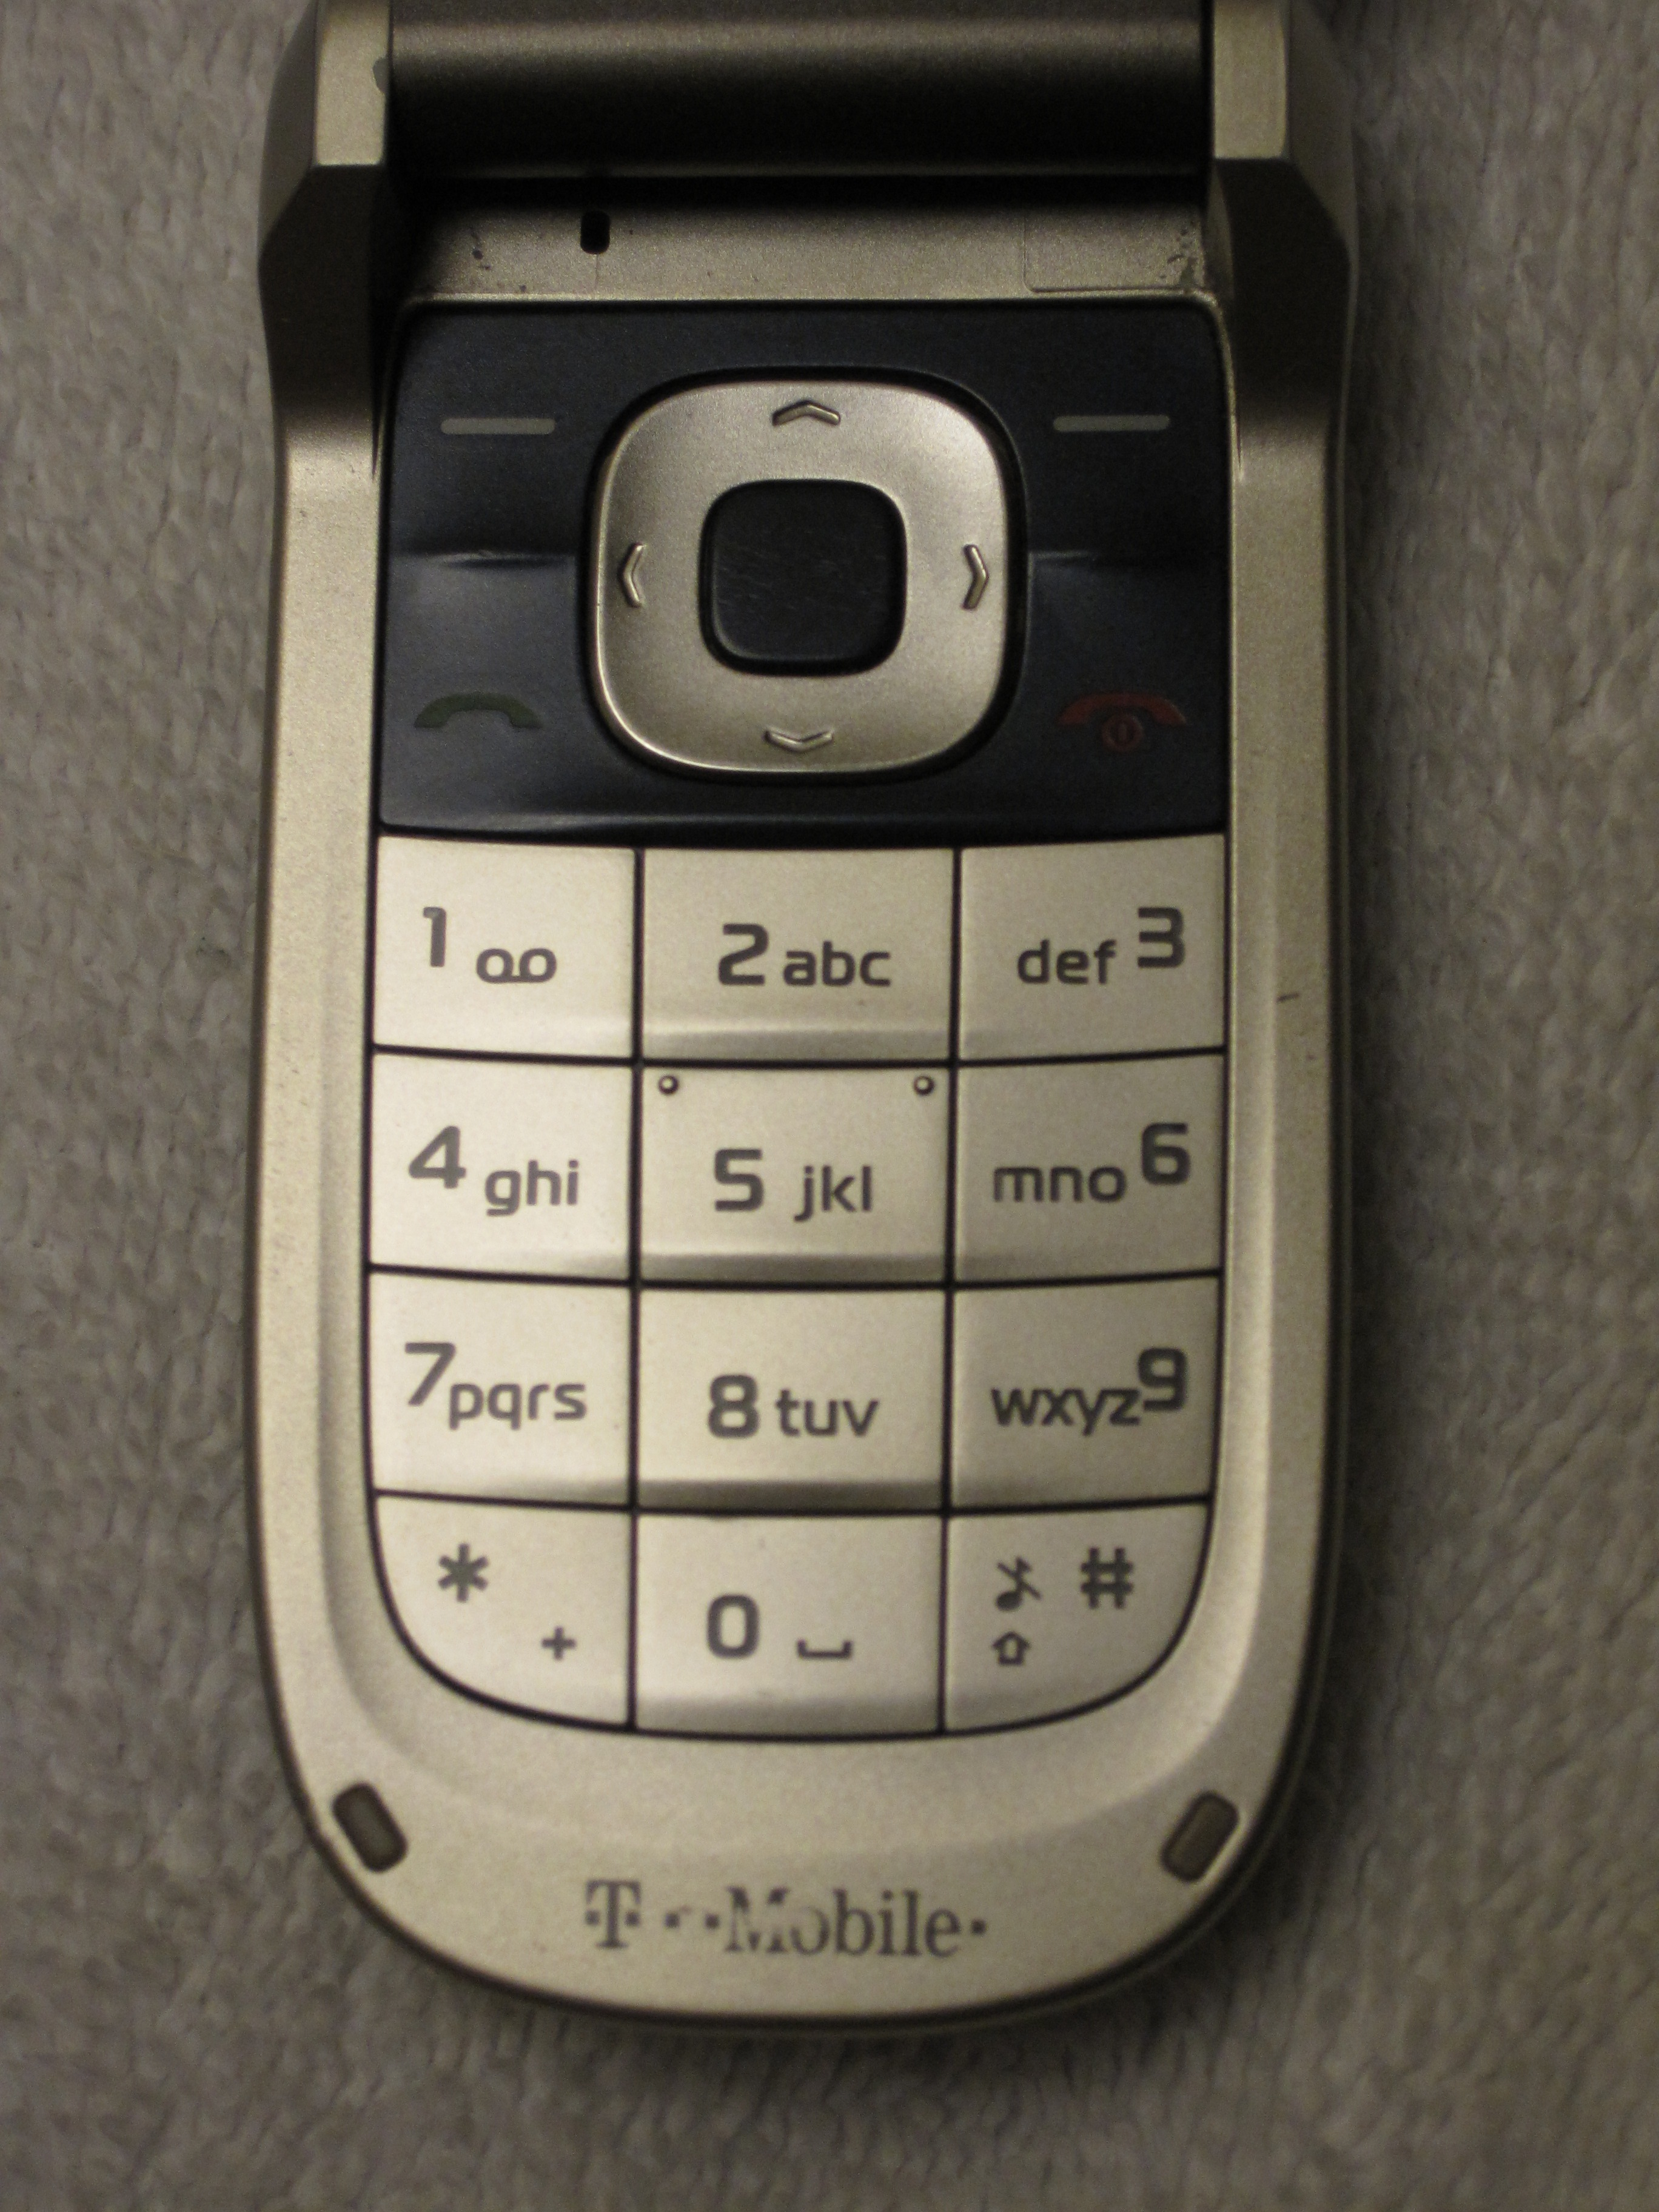
\includegraphics[width=2in]{phonekeys.jpg}
\end{center}
\caption{A cell phone keyboard}
\label{keypic}
\end{figure}

Initially, we will completely neglect the pauses and concern ourselves solely
with the number of keystrokes required.  This implies that `a' will always
require one button press, `b' will always require two, and so on.  Thus, to get
a baseline of how many keystrokes are required to enter the entirety of our
corpus of words $W$, we count the total number of occurences of each letter,
and multiply that number of occurrences by the number of button pushes
required by that letter.  Running this on the British National Corpus
using the standard cell phone keyboard layout, we find that entering the
entirety of the 100,106,029 word occurrences in the corpus would require
948,049,046 button presses.  

If we examine a cell phone keyboard (Fig.~\ref{keypic}) then we can see that
there are some terrible choices being made.  The frequently-occurring letters
'r' and 's' require more keystrokes than 'q'!  Surely, a better designed
keyboard can do better than this.  If we just reversed the order of the letters
on the 7 key, from `pqrs' to `srqp', the number of button presses required
would drop to 865,118,331 --- a savings of more than $8.7\%$!  If we assume
that every button press takes an equal amount of time, then this corresponds
the users spending $8.7\%$ less time entering their text messages.  In an
effort to find out how low this can go, we define the problem {\sc
BasicCellPhoneTyping} based on the template problem on
page~\pageref{probtemplate}.

\begin{prob}[{\sc BasicCellPhoneTyping}]~\\
\Instance\ A set of letters corresponding to an alphabet $A$ $(|A| =
n)$, a number of keys $k$, and a set of
tuples of words and frequencies $W$.  The frequencies in $W$ are integers,
and the words are made up of solely of elements of $A$. 

\Question\ What is the best partition $P$ of $A$ into $k$ sequences, such
that the total number of button presses to type every word in $W$ its
associated frequency times is minimized?  The number of button presses is equal
to the order of the letter in the sequence assigned to a given key.  For
example, in the key $2\to\{abc\}$, $a$ requires one keystroke and $c$ requires
3.  Equivalently, if we denote the number of button presses required to type
letter $a$ with partition $P$ as $\mathrm{IN}_P(a)$, then we want to find the $P$ that
minimizes $$\sum_{(w,f) \in W}\sum_{c\in w} \mathrm{IN}_P(c) * f$$
\label{bcpt}
\end{prob}

\begin{figure}
\begin{algorithm}
\Algorithm{GreedyBasicCellPhoneTyping}~$(A, k, W)$\+\\
    // $A$ is the set of letters \\
    // $k$ is the number of keys \\
    // $W$ is a set of pairs of words and their corresponding frequencies \\
    lettercount $\gets$ new\_map() \\
    \For $c \in A$\+\\
        lettercount$[c] \gets 0$\-\\
    \For (word, frequency) $\in W$\+\\
        \For $c \in$ word \+\\
            lettercount$[c] \gets $ lettercount$[c] +$frequency\-\-\\
    ordered $\gets \left[ ({\rm lettercount}[c], c)~\For c \in {\rm lettercount} \right]$\\
    sort(ordered)\\
    keys $\gets$ a array of length $k$ where each element is an empty list\\
    \For $i \gets 0 \ldots length($ordered$)$\+\\
        (count, char) $\gets$ ordered$[i]$\\
        append(char, keys$[i mod k]$)\-\\
    \Return keys
\end{algorithm}
\caption{The greedy algorithm for Prob.~\ref{bcpt}.}
\label{greedyalg}
\end{figure}

To solve {\sc BasicCellPhoneTyping} we construct a provably optimal
greedy algorithm which works in time $O(|W| + |A| \log |A|)$.  Our algorithm is
detailed in Fig.~\ref{greedyalg}, and involves creating a histogram of the
letters, and then assigning letters to keys round-robin style in the order from
most-popular to least-popular.  To prove optimality, we invoke an exchange argument.

\begin{theorem}
The greedy algorithm finds an optimal solution to {\sc BasicCellPhoneTyping}.
\label{basicthm}
\end{theorem}
\begin{proof}
We will assume, for simplicity of proof, that all letters occur a different number of times in the corpus.  
We begin by comparing two assignments of letters to keys by, for each assignment,
constructing a sequence of sets, or spectrum, $S$.  The set $S_1$ (layer 1) is the set of all
letters which require a single button press (that is, they are the first
letter in their sequence on their assigned key), $S_2$ (layer 2) is the set of
all letters which require two button presses, and so on.  If two assignments
have equal spectra, then one assignment may be transformed into
the other assignment simply by swapping letter between keys without
increasing or decreasing the total number of button pushes required to enter
the corpus of words.   Two assignments are isomorphic iff their spectra are equal.

Now assume for the sake of contradiction that we have assignment $D$, with spectrum $T$, that is not isomorphic to the greedy solution $G$ with spectrum $S$.
Note that in spectrum resulting from the greedy algorithm, all letters at layer
$i$ occur strictly more frequently than the letters at layer $j$, $j > i$.
Also, in $S$, for all layers $i$ except for the last layer, $|S_i| = k$.
Because $T$ and $S$ are not isomorphic, in $T$ there must be at least one layer $i$ such that $T_i \neq S_i$.  Let $T_i$ be the first layer for which that is true.

There are two cases for layer $T_i$.  In the first case, $|T_i| < k$, and we may
remove any element from a later layer place it in layer $T_i$ and create a strictly better layout.  In
the second case, there is some letter $a$ such that $a \in T_i$ and $a \not\in
S_i$.  We choose the least-frequent such $a$.  Because the greedy layout
algorithm creates layers in order of frequency, we know that the frequency of
$a$ is less than that of some letter $b$ in layer $T_j$, $j>i$.  Therefore, by
creating a new layout with $a$ and $b$ swapped between $T_i$ and $T_j$, we have
strictly decreased the number of button presses.  Therefore, in both cases,
$T$ was not an optimal layout, and we have reached our contradiction.
\qed
\end{proof}

For the BNC, the optimal layout has the spectrum 
$$[\{etaoinsr\}, \{hldcumfp\}, \{gwybvkxj\}, \{qz\}]$$
and any layout with that spectrum requires 638,276,114 button presses to
entire the entire BNC instead of our original requirements of
948,049,046.  This represents a savings of $32.67\%$ over our original
layout, but only for the users who type using this most basic of
input methods.  Unfortunately, this is the group of users who are likely
the least adaptable to change, as almost all ``digital natives'' use 
predictive methods to input text messages\footnote{I have no statistics
on this except for an informal survey of one of my classes.  In that
class, every student who used SMS either had a cellphone with a 26+
key alphabetic keyboard or used a predictive method.}.  In order to place the
least burden of ``newness'' on these users whilst still decreasing the number
of button presses, we now consider schemes where the only alteration of the
keyboard is the rearrangement of the sequence of letters for a given key.

By an argument symmetric to the proof of Theorem~\ref{basicthm}, we find that
the optimal layout in this new scheme is to place the letters of a given key in
sorted order, according to frequency.  Thus, the keyboard layout changes to
$2\to[acb], 3\to[edf], 4\to[ihg], 5\to[lkj], 6\to[onm], 7\to[srpq], 8\to[tuv],
9\to[wyxz]$ and requires 678,547,463 button presses to enter the whole corpus.
This represents a $28.43\%$ savings, but has the added benefit that it does not
change which key is mapped to which set of letters.  This makes it
\newword{legacy preserving}, as creating a keyboard with this layout will not
invalidate such advertising gems as 1-800-FLOWERS.  Thus, we can speed up users
by $28.43\%$ (neglecting inter-letter pauses) and not undermine 50 years of
advertising.  This layout represents perhaps the most plausible layout
yet\footnote{The described layout is the only legacy preserving layout in this
paper, and therefore should be considered the most practical suggestion.  It
also has the added benefit of not angering any of the organizations behind the
numbers 1-800-FLOWERS, 1-800-THRIFTY, and 1-800-MARINES}.  After setting up
this baseline for the easy problem, we turn our attention to optimizing
cellphone keyboards for predictive input methods.

\section{The T9 Input Method}

In an effort to minimize the pain of cellphone keyboard typing, cellular
telephone manufacturers have created the T9 input method, which attempts to
guess which letter (of the 3 or 4 possible) is intended when a user hits a
single key.  Enhancements of this input method also provide
\newword{speculative lookahead} to report, at any given time, what word it is
that the user is most likely trying to enter and provide a completion.
Unfortunately, because there are fewer keys on the cellphone keyboard than
there are letters in the English alphabet, there are words which have different
spellings but the same input sequence.  As an example, in the traditional
mapping of keys to characters both ``me'' and ``of'' have the input sequence
``63''.  Two words with the same input sequence force the user to press a third
button to cycle through the possibilities in order from most likely (``of'') to
least likely (``me'').  Even worse: ``home'', ``good'', ``gone'', ``hood'',
``hoof'', ``hone'', and ``goof'' all have the input sequence ``4663''.  If
the * key is used as the ``next match'' button, then the user will actually
have to type in ``4663******'' to type in the word ``goof'', for a total of 10
button presses --- exactly the same number of button presses required using the
default layout and the basic input method, and three more button presses than
is required when using the basic input method with an optimized layout.

When two words have the same input sequence (neglecting the *'s at the end)
then these words are \newword{t9onyms}.  When two or more words are t9onyms,
then the less-popular words require extra keypresses, raising the expected
number of keypresses to type in our corpus.  In order to type a given word, one
must press one button for every character in the word, followed by pressing
the * key as many times as there are t9onyms which are more likely than the
desired wored.  Because typing on a cellphone keyboard is already an unpleasant
experience, we would like to minimize the expected number of keystrokes.  The
number of keystrokes a word requires is equal to the number of letters in the
word, plus the number of t9onyms which are more frequent than the word.
Formally, we extend Prob.~\ref{probtemplate} and define the {\sc
MinimumT9Keystrokes} problem as:

\begin{prob}[{\sc MinimumT9Keystrokes}]~\\
\label{thm:minstrokes}
\Instance\ An alphabet $A$, a set of words and their associated frequencies $W$, and a number of keys $k$ ($|A| > k$).

\Question\ What is the partion $P$ of $A$ into $k$ sets which minimizes the total button presses required to enter the entire corpus using the T9 input method?
\end{prob}

and the corresponding decision problem is

\begin{prob}~\\
\Instance\ An alphabet $A$, a set of words and their associated frequencies $W$, a number of keys $k$ ($|A| > k$), and a number $t$.

\Question\ Is there a partition of $A$ into $k$ sets in which the total number of keystrokes required to enter the entire corpus using the T9 input method requires no more than $t$ button presses?
\end{prob}

Note that this problem is in \NP, as any assignment may be verified to require
fewer than $f$ button pushes in time proportional to the
total length of all the words in $W$.  In order to prove completeness, however,
we first prove the \NP-completeness of an intermediate problem: {\sc
UniquePathColoring}.

\begin{prob}[{\sc UniquePathColoring}]~\\
\label{upcolor}
\Instance\ A graph $G=(V,E)$, a set of paths $P$, and a parameter $k$.  A path $p$ is a sequence of vertices in which adjacent vertices in $p$ are also adjacent in the edge set $E$.

\Question\ Is there a $k$-coloring of $G$ such that every path $p\in P$ has a unique coloring?  If we consider the coloring function $\chi(v)$ to map vertices to colors, then we can extend this notation by having $\chi(p)$ map a path $p = [ v_1, v_2, \ldots ]$ to the sequence $\chi(p) = [ \chi(v_1), \chi(v_2), \ldots ]$.  Is there a coloring $\chi$ of $V$ such that 
    $$|\left\{ \chi(p)~\forall p \in P\right\}| = |P|\enspace ?$$
\end{prob}

\begin{proof}[{\sc UniquePathColoring} is \NP-complete]
To prove that {\sc UniquePathColoring} is \NP-complete, we begin by noting that any coloring of $V$ may be verified, in polynomial time, to map each path to a unique sequence of colors.  Therefore, the problem is in \NP.  To prove completeness, we reduce from {\sc GraphColoring}\cite{gandj}.

An instance of {\sc GraphColoring } consists of a graph $G=(V,E)$ and a parameter $k$.  We then ask the question of whether there is a $k$-coloring $\chi$ of the vertices of the graph such that $\forall (u,v)\in E$, $\chi(u) \neq \chi(v)$.  We transform an instance of {\sc GraphColoring} into an instance of {\sc UniquePathColoring} in the following manner:

Given $G=(V,E)$ and $k$ from {\sc GraphColoring}, we create 
$$G'=\left(V \cup \{0,1\}, E \cup \{(0,1)\} \cup \{ (v, 0)~ \forall v \in V\} \right)$$
We then uniquely number each edge in $E$ with the numbers $1 \ldots |E|$.  For each edge $e = (u,v)$ numbered $i$, we create the path set 
\begin{eqnarray*}
p_i &=& \{[v,0,b_1(i),b_2(i), b_3(i), \ldots b_{\lceil \log_2 i\rceil}], \\
    & &  ~[u, 0,b_1(i),b_2(i), b_3(i), \ldots b_{\lceil \log_2 i\rceil}]\} \\
\end{eqnarray*}
where $b_1(i)$ is the first digit of $i$ in binary, $b_2(i)$ is the second digit of $i$ in binary, and so on.  Now we create our path set 
$$P = \{ [0,1], [1,0] \} \cup \bigcup_{i = 1}^{|E|} p_i \enspace .$$
We then ask the question of whether $G'$ and $P$ can be unique-path colored using only $k$ colors.

If there is a $k$-coloring $\chi$ of $G$, then we use that coloring to generate
a $k$-unique-path coloring of $G'$ and $P$ in the following manner: First,
assign vertices $0$ and $1$ different colors from the range of $\chi$.  Next,
assign each vertex to the color it received in the $k$-coloring of $G'$.  Now,
every element of our path set corresponds to a unique color sequence.  $[0,1]$
and $[1,0]$ are the only sequences of length two, and because we assigned these
two vertices different colors, $\chi([0,1]) \neq \chi([1,0])$.  If path $x$ and
path $y$ are not from the same $p_i$, then they have a different sequence of
zeroes and ones.  Therefore, because $0$ and $1$ are assigned different colors,
the only possible path that a given path in some $p_i$ might be confused with
is the other path in that $p_i$.  But each $p_i$ corresponds to a an edge in
$E$, and we know for all edges in $(u,v) \in E$ that $\chi(u) \neq \chi(v)$.
Therefore, both paths within a given $p_i$ also have a distinct color sequence.  Therefore, given a $k$-coloring of $G$, we can generate a $k$-unique-path coloring of $G'$ and $P$.

Now we prove that given a $k$-unique-path coloring of $G'$ and $P$ we can create a $k$-coloring of $G$.
\qed
\end{proof}

However, our arbitrary remappings of the keyboard may be quickly deemed unusable.  Therefore, we define a refinement of the problem, in which the characters are required to be kept in alphabetical order as a sequence, and our only choices are about how to divide the subsequence into key assignments.  The default layout can be described as the partition $abc|def|ghi|jkl|mno|pqrs|tuv|wxyz$.  Is this partition optimal?  In order to decide this, we define the problem {\sc MinimumKeystrokePartition} as:
\begin{prob}[{\sc MinimumKeystrokePartition}]~\\
\label{thm:minpartition}
\Instance\ A sequence of letters $A = \{a_1, a_2, \ldots \}$, a set of words and their associated probabilities $W$, and a set of keys $K = \{2, 3, 4, \ldots \}$ ($|A| > |K|$).

\Question\ What is the mapping $f$ of $A \to K$ which minimizes the expected number of characters to type a word from $W$, and where $f(a_1) = 2$ and if $f(a_i) = k$, then either $f(a_{i+1}) = k$ or $f(a_{i+1}) = k+1$?
\end{prob}

As before, the corresponding decision problem is
\begin{prob}~\\
\Instance\ A sequence of letters $A = \{a_1, a_2, \ldots \}$, a set of words and their associated probabilities $W$, a set of keys $K = \{2, 3, 4, \ldots \}$ ($|A| > |K|$), and a parameter $e$.

\Question\ Is there a mapping $f$ of $A \to K$ in which the expected number of characters to type a word from $W$ is less than $e$, and where $f(a_1) = 2$ and if $f(a_i) = k$, then $f(a_{i+1}) \in \{k, k+1\}$?
\end{prob}

Again, we note that this decision problem is in \NP, as any proposed partition may be verified, in polynomial time, to have an expected value less than $e$.

\section{Exhaustive Search}

Because our problems are \NP-hard, we move on to combinatorial enumeration and experimental results.  The number of partitions of a sequence of size $n$ into $k$ subsequences is equal to $\binom{n-1}{k-1}$, and in the particular case of the 26 letter alphabet and the eight keys available on a cell phone keyboard, we find that there are $\binom{26-1}{8-1} = 480,700$ possible sequences.

\bibliographystyle{abbrv}
\bibliography{bibliography}
\end{document}
